\documentclass[12pt,a4paper,titlepage,spanish]{article} 
\usepackage{babel}
\usepackage [T1]{fontenc}
\usepackage [latin1]{inputenc}
\usepackage{graphicx}
\usepackage{amssymb}
\usepackage{amsmath}
\usepackage{setspace}
\usepackage{epsfig}
\usepackage{enumerate}
\usepackage{float}
\usepackage{array}
\usepackage{cancel}
%\usepackage{arcs}
\usepackage[usenames,dvipsnames]{color}
	  \oddsidemargin 0in
      \textwidth 6.75in
      \topmargin 0in
      \textheight 10.0in
      \parindent 0em
      \parskip 2ex
\usepackage{anysize}
\marginsize{3cm}{2cm}{1.0cm}{1.0cm}
\pagestyle{plain}
\title{
\begin{Large}
 \begin{center}
		\underline{Informe Simulaciones TP12: Modelo C�digo gen�tico} \\
		\underline{Curso: } 6to 1ra\\
		\underline{Turno: } Noche\\
		\underline{CPU: } Intel Core 2 Duo E6600\\
      \end{center}
\end{Large}
}
\author{Vileri�o, Silvio}

\begin{document}
\maketitle
\setcounter{page}{2}
\tableofcontents
\newpage

\subsection{Introducci�n}
\begin{center}
Se procede a simular un modelo de c�digo gen�tico que consiste en un ciclo de 4 partes:
\begin{itemize}
	\item a.- Generaci�n
	\item b.- Adaptaci�n
	\item c.- Cruza
	\item d.- Mutaci�n
\end{itemize}
\subsection{Generaci�n}
Sean $ N $ valores de X con $ X \in \mathbb{N} / 0 \leq X \leq 255 $ (8 bits en este caso)
Se toma una cadena de 8 bits como el ADN de los $ N $ espec�menes de la poblaci�n generada.
\subsection{Adaptaci�n funcional}
sea $ f(x)=x $ una funci�n de adaptaci�n o una funci�n ambiente que indica que bichos sobreviven:
\begin{itemize}
	\item Valores que maximizan $ y=f(x) $ sobreviven
	\item Valores que minimizan $ y=f(x) $ mueren
\end{itemize}
Se utiliz� el modelo num�rico, utilizando redondeo y m�todos de control para asegurar la poblaci�n total de N espec�menes.
Se implemento la adaptaci�n con el m�todo de las operaciones matem�ticas y los controles de redondeo(no m�todo de colas).
Sea $ F=\displaystyle\sum_{i=1}^{n} Especimen_i $ y $ N $ el total de espec�menes en la poblaci�n:
Esperanza de vida de $ Especimen_i = $  $ \frac{f(Especimen_i)}{F} $ que da un valor entre 0 y 1, si multiplicamos dicho valor por $ N $ 
obtenemos la cantidad total de espec�menes de ese tipo.
\subsection{Cruza}
Para realizar la cruza se toman dos espec�menes al azar $ \alpha $ y $ \beta $ y se les swappea una porci�n de la cadena de su ADN entre ellos.\\
Esto da lugar a nuevas especies.
\subsection{Mutaci�n}
Sea  $ M \in \mathbb{R} / 0 < X < 1 $ Se producir� una mutaci�n $ \longleftrightarrow $ $ X < 10^{-8} $
La mutaci�n consiste en invertir un bit $ (0 \rightarrow 1 ) $ o $ (1 \rightarrow 0 ) $ elegido al azar de la cadena de ADN de un espec�men tambi�n elegido al azar.
\end{center}
\subsection{Resultados}
Luego de realizar la simulaci�n, se obtuvieron los siguientes resultados: \\
\begin{itemize}
	\item Thu Oct 28 23:06:18 GFT 2010   -  Program Started.
	\item Thu Oct 28 23:06:18 GFT 2010   -  Simulation Started.
    \item	 Initial Total Poblation: 100000
	\item Thu Oct 28 23:06:19 GFT 2010   -  InitialPoblation File Creation Ended.
	\item Fri Oct 29 05:06:18 GFT 2010   -  MidPoblation File Creation Ended.
	\item Fri Oct 29 11:06:18 GFT 2010   -  Simulation Ended.	
	\item Fri Oct 29 11:06:19 GFT 2010   -  FinalPoblation File Creation Ended.
	\item Fri Oct 29 11:06:19 GFT 2010   -  Histograms File Creation Ended.
	\item Mutation Count: 4
	\item Final Total Poblation: 100000
\end{itemize}
\begin{center}
	Histograma inicial\\
	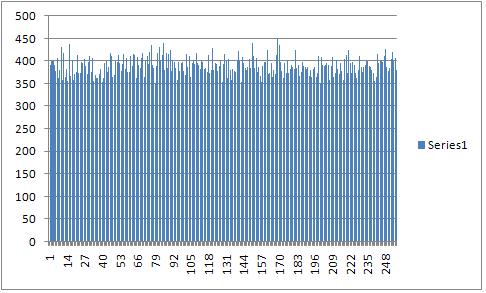
\includegraphics[scale=1.00]{images/inicial.jpg}
\end{center}
\newpage
\begin{center}
    Histograma intermedio\\
	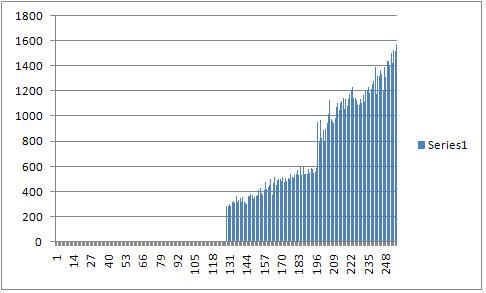
\includegraphics[scale=1.00]{images/intermedio.jpg}
\end{center}
\begin{center}
    Histograma final\\
	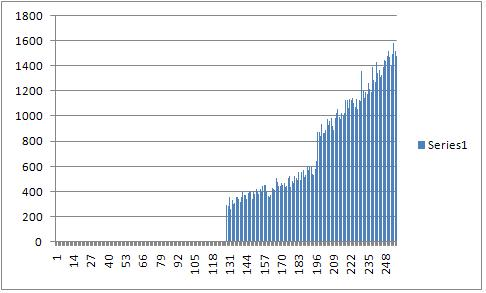
\includegraphics[scale=1.00]{images/final.jpg}
\end{center}
\newpage
\subsection{Conclusi�n}
Se puede observar que luego de un tiempo, se acent�a la poblaci�n de los espec�menes mas fuertes o con mas valor, y que los de valores peque�os desaparece por completo.
Las mutaciones, provocan cambios repentinos en la poblaci�n.
\end{document}